\chapter{Stand der Technik}
\label{chap:technikStand}
%\section{Theorien}
%\section{Techniken}
    Zur Analyse des aktuellen Standes der Technik und Forschung in Bezug zur Konzeption von Software-Lösungen, mit denen 
    die formalisierten Interaktionen der Softwareentwickler vereinfacht werden können, erfolgt in diesem 
    Kapitel ein systematisches Literaturreview. Die Literaturprüfung wird gemäß den Richtlinien, die in der Publikation 
    von \cite{Kitchenham2007} vorgeschlagen werden, durchgeführt. 

    %\section{Methodiken}
    %\label{sec:methodiken}
    %    Im Rahmen dieser Arbeit wurden zur Informationserhebung zuerst ein systematisches Literaturreview durchgeführt und

    \section{Systematisches Literaturreview}
    \label{subsec:systematischesLiteraturReview}
        Die Thematik des systematischen Literaturreviews wurde bereits in den einleitenden Kapiteln erwähnt. 
        Dieser Abschnitt widmet sich ausschließlich der Anwendung der Richtlinien und dem daraus abgeleiteten Stand der Technik 
        abhängig zu dem in der Arbeit behandelten Thema. 

    \subsection{Ziele des Systematischen Literaturreviews}
        Das Ziel dieses systematischen Literaturreviews ist es, die aktuellen Fortschritte von Smart Home Plattformen und 
        Gateways in Richtung der entwicklerseitigen Benutzerfreundlichkeit zu recherchieren. Dabei liegt der Schwerpunkt 
        auf der Usability und der einfachen Handhabung der formalisierten Interaktionen der Softwareentwickler. Es gilt zu 
        analysieren, ob es in diesem Themenbereich bereits Publikationen und Forschungen gibt und welche Entscheidungen 
        getroffen werden müssen, um die Weiterentwicklung eines Systems nicht je nach hinzukommender Funktionalität oder 
        auch Bedingung komplexer werden zu lassen. Die Ergebnisse dieses systematischen Literaturreviews sollen daraufhin 
        als Grundlage der Konzeption einer solchen Plattform dienen und mit einfließen. 

    \subsection{Suchstrategie- und anfragen}
        Dieser Abschnitt beschreibt die Suchstrategie und die Anfragen zu dem systematischen Literaturreview. Hierbei wird 
        erläutert, anhand welcher Kriterien die Literatur ausgewählt wird.
        \\
        In den ersten Schritten werden anhand der Forschungsfragen in Kapitel (\ref{sec:forschungsfragen}) die Stichpunkte 
        aufgegriffen und als Suchterm formuliert. Die daraus resultierenden Suchterme, die der tabellarischen Darstellung 
        (\ref{tab:slr}) zu entnehmen sind, werden in diversen wissenschaftlichen Fachdatenbanken recherchiert und analysiert. 
        Die Ergebnisse werden nach ihrem Titel und der Zusammenfassung sortiert. Gibt es Publikationen mit vergleichbaren 
        Inhalten, so sind diese in weiteren Schritten näher zu betrachten. Damit die Literaturrecherche weitere Ergebnisse 
        erzielt, wird beim studieren der Publikationen die Schneeballsuche angewendet. Dabei wird in den Quellen der jeweiligen 
        Literatur auf weitere Verweise geschaut, die ebenso potentielle Inhalte bearbeiten. Die Kombination beider 
        Literaturergebnisse bilden die Grundlage der zu analysierenden Quellen und geben so den Stand der Technik wieder.
        \begin{figure}[hbt!]
            \centering
            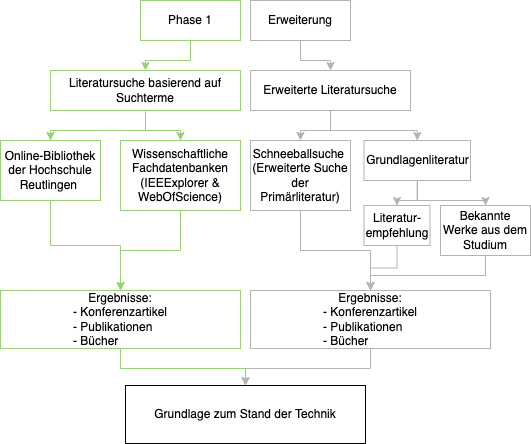
\includegraphics[width=13cm,height=13cm,keepaspectratio]{images/slr_walkthrough.png}
            \caption{Strategie der Literatursuche}
            \label{fig:slr}
        \end{figure}
        \\
        Die generierten Suchterme, die daraus resultierenden Literaturergebnisse und der damit einhergehende Suchverlauf ist 
        zur Nachvollziehbarkeit tabellarisch aufgeführt:
        \\
        \linebreak
        \pagebreak
        \begin{table}[hbt!]
            \begin{center}
                \begin{tabular}{| p{2.9cm} | p{1.9cm} | p{1.6cm} | p{1.9cm} | p{1.9cm} | p{1.8cm} | p{1.8cm} | }
                    \hline
                        \textbf{Suchanfrage} & \textbf{Datum} & \textbf{Filter} & \textbf{Plattform} & \textbf{Ergebnisse} & \textbf{Gesehene} & \textbf{Relevant} \\
                    % \hline
                        % formalized interactions software development & 08.04.2022, 03.05.2022 & Nein & IEEExplorer, WebOfScience & 55, 106 & 5, 4 & 0, 0 \\ 
                    \hline
                        formalized interactions software development architecture  & 11.04.2022, 03.05.2022 & Nein & IEEExplorer, WebOfScience & 13, 26 & 6, 4 & 0, 0 \\ 
                    \hline
                        usability AND formalized interactions AND architecture & 11.04.2022, 03.05.2022 & Nein & IEEExplorer, WebOfScience & 3, 7 & 1, 3 & 0, 1 \\ % A Conceptual Model of Service Customization and Its Implementation
                    \hline
                        usability AND formalized interactions AND architecture AND smart home & 01.05.2022 & Nein & IEEExplorer, WebOfScience & 0, 0 & 0, 0 & 0, 0 \\
                    \hline
                        usability AND formalized interactions AND software development AND architecture & 02.05.2022 & Nein & IEEExplorer, WebOfScience & 1, 1 & 1, 1 & 0, 1 \\
                    \hline
                    %    usability AND formalized interactions AND software development AND architecture AND smart home & 02.05.2022, 03.05.2022 & Nein & IEEExplorer, WebOfScience & 0, 0 & 0, 0 & 0, 0 \\
                    %\hline
                        usability AND architecture AND gateway AND smart home & 06.05.2022 & Nein & IEEExplorer, WebOfScience & 2, 4 & 1, 1 & 1, 1 \\
                    \hline
                        usability AND formalized interaction AND (architecture OR smart home OR software developer OR gateway) & 09.05.2022 & Nein & IEEExplorer, WebOfScience & 3, 10 & 1, 2 & 0, 0 \\
                    \hline
                        usability AND architecture AND smart home AND (formalized interaction OR software developer OR iot) & 09.05.2022 & Nein & IEEExplorer, WebOfScience & 13, 22 & 3, 3 & 0, 0 \\
                    \hline
                \end{tabular}
            \end{center}
            \caption{Suchprotokoll des Systematischen Literaturreviews}
            \label{tab:slr}
        \end{table}
    \subsection{Datenextraktion und Synthese}
        Zu der zielgerichteten Datenextraktion werden in Anlehnung an die Richtlinien des systematischen Literaturreviews die folgenden 
        Einschluss- und Ausschlusskriterien definiert, die dabei helfen, die relevanten Publikationen zu finden:
        \begin{table}[hbt!]
            \centering
            \begin{tabular}{p{0.125cm} p{15cm}}
                    \textbf{\#} & \textbf{Einschluss-Kriterien}\\ 
                \hline
                    1  & Die Literatur ist in den wissenschaftlichen Fachdatenbanken veröffentlicht, darunter: WebOfScience, IEEExplorer, SpringerLink, Elsevier, Addison-Wesley, dpunkt-Verlag, ACM und Google Scholar  \\ 
                \hline
                    2  & Der Beitrag wurde nach 2010 veröffentlicht \\ 
                \hline
                    3  & Die Veröffentlichung ist in deutscher oder englischer Sprache \\
                \hline
                    \textbf{\#} & \textbf{Ausschluss-Kriterien}\\ 
                \hline
                    1  & Die Veröffentlichung beinhaltet, bzw. behandelt nicht die Schlagworte usability, architecture, formalized interaction oder iot \\ 
                \hline
                    2  & Die Publikation gehört zu der Literatur der Grauzone \\ 
                \hline
                    3  & Die Veröffentlichung hat weniger als 5 Zitationen \\
                \hline
                    4  & Die Literatur hat weniger als 5 Seiten Inhalt \\
            \end{tabular}
            \caption{Einschluss- und Ausschlusskriterien des systematischen Literaturreviews}
            \label{tab:slr_criteria}
        \end{table}
        \\
        Mit der Forschungsfrage, den Suchtermen und den Einschluss- und Ausschlusskriterien zu der Quellenrecherche werden während der Anwendung
        des systematischen Literaturreview-Templates und deren Richtlinien die erzielten Ergebnisse synthetisiert und zusammengefasst. Im Rahmen 
        dieser Forschungsfrage und der Auslegung der Suchterme, die in Tabelle (\ref{tab:slr}) zu entnehmen sind, ergab sich nicht die Menge an Literatur, 
        die notwendig ist, um ein umfangreiches Literaturreview im Stil des Templates durchzuführen. Demnach ist kein vollständiges systematisches Literaturreview 
        möglich. Die wenigen relevanten Ergebnisse des Literaturreviews geben einen Einblick in Bereiche, die als Gedankenanstoß und zum transferieren von 
        Wissen, Gedanken und Ideen geeignet sind. 
        \\
        \linebreak
        Unter der Betrachtung des Resultats des durchgeführten Literaturreviews gilt die Forschungsfrage als innovativ und eröffnet eine 
        neue Sichtweise basierend auf der Literatur. Um dennoch eine fundierte wissenschaftliche Grundlage zu repräsentieren, wird in 
        folgendem Abschnitt auf Referenzen und Literatur eingegangen, die Teile der Forschungsfrage abdecken und mehr als Gedankenanstoß 
        anzusehen sind, beziehungsweise auch einen partiellen Einblick in den Stand der Technik bieten. 
%\pagebreak
\section{Zusammenfassung} 
    Speziell auf die Forschungsfrage in Kapitel (\ref{sec:forschungsfragen}) gibt es in dem heutigen Stand der Technik keine explizite 
    Literatur, welche den Gedanken aufgreift und behandelt. Die Literatur, die bei dem systematischen Literaturrecherche erarbeitet wurde, 
    deckt trotz dessen manche Aspekten ab, die interessante Anhaltspunkte und Ideen thematisieren. Diese geben Impulse und helfen bei den weiteren 
    Schritten in dieser Arbeit hinsichtlich der Konzeption. 
    
    \subsection{Publikationen}
    \label{subsec:publications}
        Im Folgenden wird die relevante Literatur aufgegriffen und zusammengefasst, sodass ein Einblick in den Prozess der 
        Informationserhebung, der Sammlung von Erfahrungswerten und Ideen gewährleistet wird.
        
        \subsubsection*{Design and Realization of a Framework for Human-System Interaction in Smart Homes}
            In dem Artikel von \cite{Wu2012} wird zu Anfang die Beziehung zwischen Benutzern, Räumlichkeiten und 
            Diensten analysiert. Basierend auf den daraus gewonnenen Erkenntnissen wird ein Framework und ein 
            entsprechender Algorithmus vorgestellt, welcher die Interaktionsbeziehungen modelliert. Basierend auf den  
            Ergebnissen wird ein Framework entwickelt, welches die Interaktionsanforderungen abdeckt. Hauptmerkmale 
            waren dabei Komfort, Bequemlichkeit und Sicherheit. Zur abschließenden Überprüfung des Designkonzeptes und 
            der Implementierung wurden Probanden zum Testen der Anwendung ausgewählt und anschließend ein Interview 
            durchgeführt. Das Evaluierungsergebnis zeigt, dass das Framework eine gute Einführung in die Verbesserung 
            der Mensch-System-Interaktionen darstellt. 

        \subsubsection*{Seamless Integration of Heterogeneous Devices and Access Control in Smart Homes}
            Der Artikel von \cite{Kim2012} erarbeitet einen Vorschlag einer ganzheitlichen und erweiterbaren 
            Softwarearchitektur, welches Dienste und heterogene protokoll- und herstellerspezifische Geräte 
            nahtlos integrieren lässt und Sicherheit über das Internet gewährleistet. Grundlegend wird hierbei auf das 
            \acs{OSGI} Framework gesetzt. Dadurch wird die semantische Interoperabilität hervorgehoben. Dies ist die Fähigkeit, 
            neue Anwendungen und Treiber zur Laufzeit in das bereitgestellte System zu integrieren \cite{Kim2012}. 
            Zusätzlich zu dem System wird im Rahmen dieser Publikation ein Zugangskontrollmodell für spezielle \acl{SH} 
            Szenarien integriert. Zur Beweisführung wird das Konzept anhand von semantischen Erkennungen von Heimgeräten zur 
            Laufzeit demonstriert. Dafür werden mehrere Protokolle, darunter X10, ZigBee und Insteon, in einen realen Test 
            integriert. Die Arbeit behandelt die folgenden Schwerpunkte \cite{Kim2012}:
            \begin{itemize}
                \item Analyse einer Reihe von Heimnetzprotokollen hinsichtlich ihrer Erkennungs- und Integrationsanforderungen.
                \item Eine erweiterbare Home-Gateway-Architektur, die es ermöglicht, heterogene Geräte während der Laufzeit flexibel zu installieren, zu verwalten und darauf zuzugreifen.
                \item Ein neuartiger Zugangskontrollmechanismus speziell für Smart-Home-Systeme.
                \item Die Umsetzung des vorgeschlagenen Konzepts, indem gezeigt wird, wie verschiedene Geräte integriert und von Endbenutzern aufgerufen werden können.
            \end{itemize}
            Die Architektur und die damit eingesetzte semantische Abstraktionsschicht unterstützt laut den Ergebnisse 
            erheblich die Anwendungsentwicklung. 
            \\
            Mit der Zugriffskontrollrichtlinie wird den Hausbesitzern eine stabile Kontrolle darüber gegeben, mit der 
            die Benutzer auf die smarte Geräte zugreifen können. Das Resultat dieser Arbeit scheint zu zeigen, dass damit 
            die Barriere für \acl{SH} Systeme gesenkt wird. 

        \subsubsection*{Wireless Architectures for Heterogeneous Sensing in Smart Home Applications: Concepts and Real Implementation}
            Dieser Beitrag von \cite{Viani2013} diskutiert die aktuellen Trends von drahtlosen Architekturen für Anwendungen 
            im \acl{SH} Bereich. Aus der Diskussion wurden Vorteile erarbeitet, die anschließend über die Verwendung der 
            drahtlosen Architektur analysiert wurden. Schwerpunkt dabei lag jedoch auf der Schätzung des Benutzerverhaltens. 
            \\
            \linebreak
            Allgemein behandelt der Artikel die Vorstellung einer drahtlosen Architektur für intelligentes Energiemanagement 
            und die Überwachung von älteren Menschen, indem die Anwesenheit, die Bewegung und das Verhalten der Bewohner 
            analysiert wird \cite{Viani2013}. 
            \\
            Interessant dabei ist das entstandene Konzept der konkreten Softwarearchitektur.

        \subsubsection*{My House, My Rules: A Private-by-Design Smart Home Platform}
            Dieses Whitepaper von \cite{Zavalyshyn2020} stellt eine \textit{Private-by-Design-IoT-Plattform} für \acl{SH} 
            Umgebungen vor. Mit dem Konzept wird eine typische Architektur für bestehende \acs{IoT} Plattformen als Grundlage 
            verwendet, die über ein alternatives Design mehr Sicherheit und Kontrolle für den Hauseigentümer bietet. 
            Genutzt wird dabei die von Intel entwickelte \ac{SGX}\footnote{Eine hardwarebasierte Verschlüsselung von Speicherinhalten, die bestimmten Programmiercode und Daten im Speicher isoliert. \url{https://www.intel.de/content/www/de/de/architecture-and-technology/software-guard-extensions.html} Abgerufen am 15.05.2022.}. 
            Diese Erweiterung ermöglicht es, eine intuitive Sicherheitsabstraktion einzuführen, die den unbefugten Zugriff auf Daten 
            durch nicht vertrauenswürdige \acs{IoT} Cloud-Anbieter verhindert. Das Konzept wurde in einen Prototyp umgesetzt und 
            evaluiert. Dabei wurden auch eine quantitative Forschung durchgeführt, die aus mehr als 40 Probanden bestand, welche 
            den Prototypen verwendet und anschließend bewertet und beurteilt haben. Die Mehrzahl der Teilnehmer der Feldstudie 
            hielten die Softwareplattform als benutzerfreundlich und die unterstützen Richtlinien durch die Sicherheitsabstraktion 
            für nützlich \cite{Zavalyshyn2020}. Mit den Richtlinien kann verstärkt die Privatsphäre der Anwender in ihrem Wohnraum 
            geschützt werden. Der Sicherheitsmonitor der Software ermöglicht Endbenutzern eine granulare Kontrolle und Überwachung 
            der Datenflüsse, die durch die \acs{IoT} Geräte generiert werden, sowie die Verhinderung von potentiellen 
            Datenschutzverletzungen der Hersteller durch die Verwendung einer Datenschutzrichtlinie. 

        \subsubsection*{Fast-prototyping Approach to Design and Validate Architectures for Smart Home}  
            Inhalt des Artikels von \cite{Montanaro2021} ist das Entwickeln eines komplexen \acl{SH} Systems. 
            Hintergrund dafür ist die kontinuierliche Entwicklung und Kommerzialisierung sämtlicher \acs{IoT} Geräte und 
            die damit einhergehende Änderung oder Anpassung der Nutzeranforderungen. Dadurch benötigt die Community eine 
            schnelle Lösung, bzw. einen Prototypen, um die Anforderungen der Nutzer zu erfüllen und auf schnell 
            entstehenden Notwendigkeit vorbereitet zu sein. 
            \\
            Grundlage für die Entwicklung der Plattform ist eine aktuelle und solide Studie, die ebenso im Rahmen des 
            Artikels durchgeführt wurde. Die Benutzeranforderungen wurden aus der Studie extrahiert und sind bei der 
            Planung des Konzeptes mit eingeflossen. Bestandteil dieser Arbeit ist unter anderem die Verwendung von Node-RED\footnote{Ein von IBM entwickeltes grafisches Entwicklungswerkzeug mit Baukastenprinzip. Funktionsbausteine können per Verbindungen miteinander verknüpft und als Prozess bearbeitet werden. \url{https://nodered.org/} Abgerufen am 15.05.2022.} und 
            dem \acs{MQTT} Kommunikationsprotokoll. 
            \\
            \linebreak
            Die in der Arbeit vereinfachten formalisierten Interaktionen werden speziell dem Anwender gegenüber durch 
            Node-RED visualisiert und die komplexe Logik somit vereinfacht dargestellt. Die Idee mit dem Verwenden von Node-RED 
            ist ein guter Gedanke der formalisierten Interaktionen und kann auch dem Entwickler programmatisch Schritte 
            erleichtern. Da selbst das Framework verstanden werden muss, ist eine gewisse Komplexität nicht zu verhindern. 
            Dennoch kann der Gedanke in weiteren Forschungsschritten weitergedacht oder optimiert werden. Mit diesem 
            Grundsatz sind gute Lerneffekt zu erzielen, indem diese Technologie zu praktischen Arbeiten im Forschungs- und 
            Bildungsbereich eingesetzt wird. 
    \\
    \linebreak
    Alle oben aufgeführten Artikel und Forschungsarbeiten sind keine explizite Referenz, bzw. stehen in keinem vollumfänglichen 
    Verhältnis zu der in dieser Arbeit gestellten Forschungsfrage, da mit dem systematischen Literaturreview keine Literatur 
    gefunden werden konnte, die sich ausschließlich dem zu behandelnden Thema widmet. Die zusammengefassten Arbeiten dienen 
    lediglich als stichpunktartige Übersicht, um einen Einblick zu gewährleisten, welche Forschungsarbeiten mit den 
    Suchtermen (siehe Tabelle \ref{tab:slr}) erzielt wurden. Basierend auf diesen Grundlagen und dem damit vermittelten Wissen 
    konnten unter anderem die Anforderungen verfeinert und gefestigt werden, sowie Ideen für das folgende Konzept in Kapitel 
    (\ref{chap:konzept}) aufgegriffen werden.
    \\ 
    Durch das systematische Literaturreview wird deutlich, dass der Stand der Technik in die Richtung, in die die Arbeit 
    abzielt, keine aussagekräftigen Ergebnisse zeigt. Mittels weiteren Experten Interviews wird deutlich, dass viele mit der 
    Thematik des \acl{SH} vertraut sind, jedoch überwiegend nur als Anwender bestehender Plattformen und Geräte gelten.
    \\
    Die mit den Experten Interviews erlangten Informationen sind nicht repräsentativ, lediglich eine Erkenntnis im Rahmen 
    dieser Arbeit.
    \\
    Um einen Gesamtüberblick bezüglich dem Technikstand rundum \acl{SH} zu vermitteln, 
    wird in folgendem aus einer etwas pragmatischeren Sichtweise der Stand der Technik skizziert.
    
    \pagebreak
    \subsection{Stand der Technik aus Nutzer- und Produktsicht}
        Der aktuelle Markt bietet bereits viele Möglichkeiten und Alternativen der Umsetzung eines intelligenten Zuhause. 
        Darunter z.B. kommerzielle in sich geschlossene Systeme, die ausschließlich dem Nutzer als Anwendung verkauft werden, 
        einzelne Intelligente Geräte, die nichts zwangsläufig eine zentrale Plattform benötigen und Plattformen, wie bspw. 
        Home Assistant und openHAB, die eine gewisse Technikaffinität erfordern und voraussetzen, um diese nach belieben 
        einsetzen und konfigurieren zu können. Viele große Unternehmen, darunter Bosch, Telekom, Siemens, Samsung und viele mehr bieten Geräte 
        und Softwarelösungen, die der Nutzer als reine Anwendung benutzt, an. Diese geben keinen Einblick in ihre Software 
        und deren Umsetzung, daher sind diese zum Vergleich nicht weiter zu berücksichtigen. 
        \\
        \linebreak
        Neben den bekanntesten, frei verfügbaren Plattformen openHAB und Home Assistant gibt es weitere Lösungen, die eine 
        Platform zur Verfügung stellen\footnote{Aufstellungen von verfügbaren Open Source Smart Home Plattformen im Jahr 2020. \url{https://ubidots.com/blog/open-source-home-automation/} Abgerufen am 16.05.2022}:
        \begin{itemize}
            \item OpenMotics
            \item Jeedom
            \item ioBroker
            \item AGO Control 
            \item Domoticz
            \item Homebridge.io
        \end{itemize}
        Neben den aufgelisteten Produkten gibt es noch weiter, die jedoch nicht weiter aufgeführt werden. 
        Durch die Vielzahl der Angebote und den immer größer werdenden Mehrwert, den eine solche Plattform bietet, 
        nimmt die Forschung und Entwicklung in dem Bereich des \acs{IoT} zu. Dadurch können immer mehr 
        Anwendungsfälle abgedeckt und realisiert werden, wodurch dem Nutzer die Einsatzmöglichkeiten deutlicher 
        und effektiver erscheinen. 
        Dies wird in Kapitel 
        (\ref{chap:anforderungsanalyse}) durch die konkrete Marktanalyse (siehe Abschnitt \ref{sec:marktanalyse}) deutlich. 
        % Ergänzung um CommandLine Tools, die dem Entwickler helfen auf zentraler Ebene (ng generate, GitHub Copilot, 
        % Code completion, code generation etc.)